\newpage
\chapter{ОСОБЕННОСТИ АДАПТИВНОЙ ПОТОКОВОЙ ПЕРЕДАЧИ ВИДЕОДАННЫХ В ТЕЛЕКОММУНИКАЦИОННЫХ СЕТЯХ}
\label{chap1}

\section{Вводные замечания}

В течение последних лет наблюдается существенное развитие телекоммуникационных систем, особенно сетей мобильной связи. Это проявляется в росте скоростей передачи данных в каналах связи и увеличении числа обслуживаемых устройств в сети. Увеличение производительности мобильных устройств позволяет им обрабатывать больший объем информации и приводит к увеличению нагрузки на беспроводные сети. Наибольшей популярностью среди пользователей мобильных сетей попользуются сервисы просмотра видеоконтента по протоколу HyperText Transfer Protocol (YouTube, Vimeo и т. д.) плотно интегрированные с социальными сетями. Подобное явление приводит к колоссальному росту нагрузки на существующие мобильные сети. Следует отметить, что за 2016-й год объем передаваемой информации через телекоммуникационные мобильные сети увеличился на 63 процента и доминирующим видом передаваемой информации является видеоконтент, который занял 60 процентов объема трафика, прошедшего через мобильные сети. По прогнозам ведущих производителей сетевого оборудования видеоданных, займет около 78-ми процентов всего мобильного трафика к 2021-му году~\cite{Cisco}.

Основной проблемой сетей мобильной связи является ограниченность доступной частотной полосы для организации беспроводного канала, что приводит к ограничениям на пропускную способность каналов связи и число абонентов, одновременно активных в сети. Увеличение объема трафика в сети негативно влияет на качество обслуживания абонентов, наиболее сильно выражающегося в уменьшении скорости передачи информации, увеличении среднего значения и дисперсии задержки при доставке данных абоненту. Наиболее чувствительной, к данным факторам обслуживания, является передача видеоданных. Как следствие, операторы мобильной связи и производители телекоммуникационного оборудования ищут пути оптимизации совместной передачи различных видов трафика в существующих и разрабатываемых системах, где наибольшим приоритетом обладает именно передача видеоданных.

Для организации исследования в области передачи видеоданных важным является установление ключевых показателей производительности сети передачи информации и критерия качества восприятия с позиции доставки видеоконтента. Основным критерием производительности сетей передачи видеоданных является именно критерий качества восприятия~--~субъективная реакция пользователя на характеристики воспроизведения видеопоследовательности. Важной отличительной чертой передачи видеоданных является влияние на качество восприятия особенностей работы воспроизводящего устройства, называемого видеоплеером.

Данный раздел посвящен рассмотрению особенностей передачи видеоданных в современных телекоммуникационных сетях и организован следующим образом. В начале рассматривается система передачи видео в целом и описывается формат хранения видеопоследовательностей. Далее производится анализ существующих видеоплееров, и на его основе предлагается модель генерируемого трафика при просмотре видео. В заключении производится обзор ключевых показателей производительности телекоммуникационных сетей и методик оценки качества восприятия при передаче видеоданных.

Ввиду большого числа англоязычных терминов, используемых в данном разделе, далее представлен список основных используемых сокращений, их расшифровок и кратких описаний.
\begin{itemize}
  \item Key Performance Indicators (KPI)~--~ключевые показатели производительности;
  \item Quality of Experience (QoE)~--~критерий качества восприятия;
  \item Mean Opinion Score (MOS)~--~усредненное мнение по группе пользователей;
  \item Transmission Control Protocol (TCP)~--~протокол транспортного уровня для гарантированной доставки информации;
  \item Media Presentation Description (MPD)~--~формат файла, описывающий представление видеопоследовательности на сервере;
  \item HyperText Transfer Protocol (HTTP)~--~протокол прикладного уровня для обмена информации в телекоммуникационных сетях;
  \item HTTP Progressive Download (HPD)~--~неадаптивная технология передачи видеоданных;
  \item HTTP Adaptive Streaming (HAS)~--~адаптивная технология передачи видеоданных;
  \item Moving Picture Experts Group~-~Dynamic Adaptive Streaming over HTTP (MPEG-DASH)~--~международный стандарт передачи видеоданных, поддерживающий адаптацию видеопотока.
\end{itemize}

\section{Структура систем передачи видеоданных}\label{chap1:SystemStructure}

Современные системы передачи видеоданных по протоколу HyperText Transfer Protocol состоят из трех основных компонентов (рисунок~\ref{fig:Base_Scheme}):

\begin{itemize}
  \item Видео Контент Сервер~--~программно-аппаратный комплекс обеспечивающий хранение и доступ к видеоданным;
  \item Сеть передачи информации~--~среда передачи информации, организующая соединие между узлами сети;
  \item Пользовательское устройство~--~программно-аппаратный комплекс производящий загрузку и демонстрацию видео пользователю.
\end{itemize}

\begin{figure}[htbp]
\begin{center}
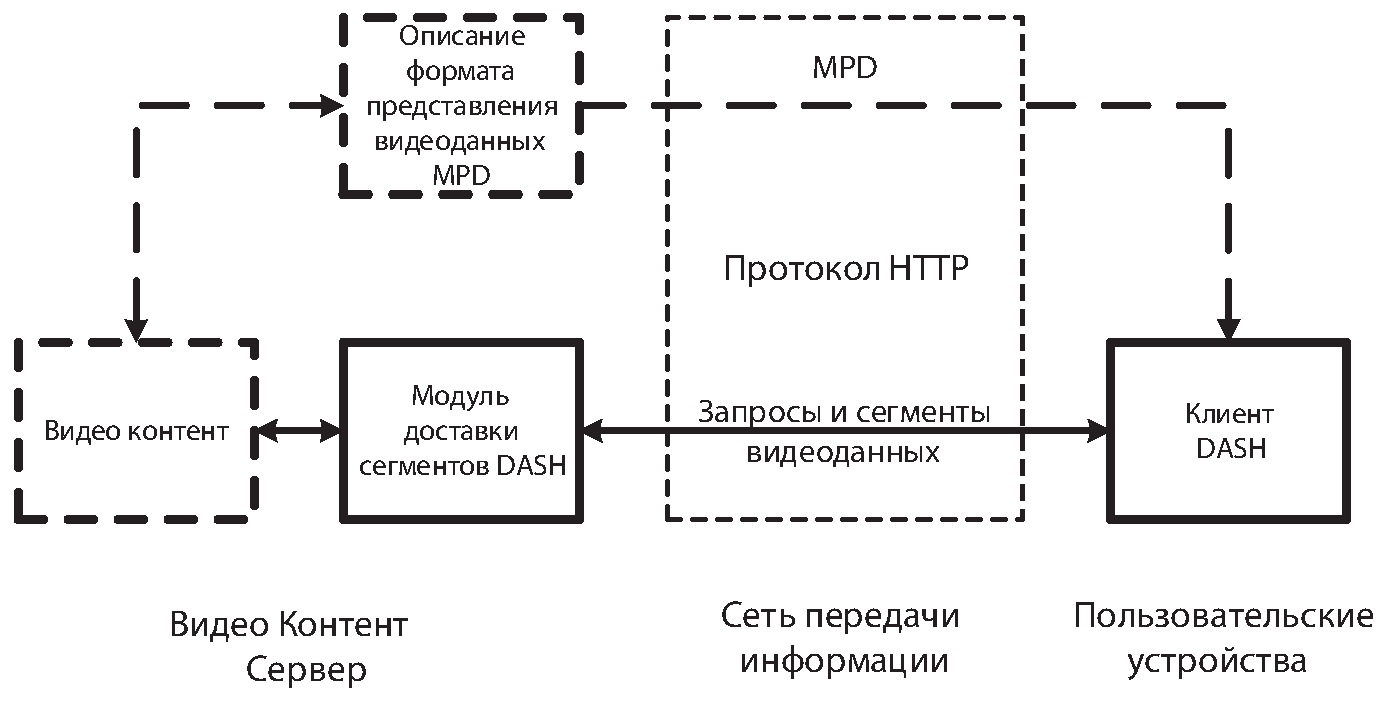
\includegraphics[width=0.8\textwidth]{Chapter1/Base_Scheme.pdf}
\caption{Обобщенная структура систем передачи видеоданных}
\label{fig:Base_Scheme}
\end{center}
\end{figure}

При передаче видеоданных удаленно в сети Интернет установлена система серверов (Видео Контент Сервер), хранящая видеоданные. К данной системе посредствам HyperText Transfer Protocol (HTTP), HyperText Transfer Protocol Secure (HTTPS) или Transport Layer Security (TLS) протоколам через сеть передачи информации подключаются пользовательские устройства. При установке соединения с каждым пользователем производится формирование сессии по протоколу гарантированной доставки данных TCP (Transmission Control Protocol). Данный протокол обеспечивает надежную передачу информации между узлами сети за счет использования дополнительных сообщений, подтверждающих доставку данных (квитанций). Важно отметить, что загрузкой видеоданных управляет программный комплекс, установленный на пользовательском устройстве~--~видеоплеер. Именно видеоплеер принимает решение о порядке загрузки данных путем формирования последовательности запросов на сервер хранения информации в зависимости от воспроизведения и статистики получения информации.

Исходя из специфики работы работы сетевых протоколов HTTP и TCP, при прохождении через сеть передачи информации происходит только задержка данных при доставке на пользовательское устройство. Как следствие, невозможна ситуация, когда происходит потеря данных при передаче через сеть. Важной особенностью систем, основанных на протоколе HTTP, является их инвариантность к сети передачи информации: для обеспечения работы такой системы необходима лишь корректная работа протокола HTTP и нижележащих уровней. Однако, использование на транспортном уровне протокола TCP вносит небольшую избыточность, обусловленную квитированием и повторными передачами данных.

Задержка при передаче информации может привести к появлению негативных эффектов воспроизведения, таких как длительное время ожидания начала проигрывания, остановка воспроизведения ввиду недостатка загруженных данных и, как следствие, уменьшению удовлетворенности пользователя просмотром.

Целью данного раздела является именно установление взаимосвязи между характеристиками сети передачи информации и удовлетворенностью пользователя проигрыванием потока, прошедшего через нее. На основе данной взаимосвязи возможно построить решения для увеличения производительности телекоммуникационных сетей для передачи видеоданных. Первым шагом для достижения поставленной цели является рассмотрения формата представления видео информации при передаче через телекоммуникационные сети.

Основные результаты данного раздела опубликованы в работе \cite{past_ius}.

\section{Представление видеоданных при передаче через телекоммуникационные сети}
\label{chap1:VideoFormat}

Опишем формат хранения информации на Видео Контент Сервере для передачи с использованием HTTP протокола. Каждая последовательность, хранящаяся в памяти сервера, разбита на периоды равной длительности называемыми сегментами (в англоязычной литературе Segments или Chunks). Каждый сегмент характеризуется уникальным идентификатором (порядковым номером и идентификатор видео) и репрезентацией~\cite{dash_standard}.

Репрезентация является общепринятой характеристикой видеопотока. Она включает в себя три параметра:
\begin{itemize}
  \item Битовая скорость потока~--~объем информации, необходимый для хранения данных в одну единицу времени. Общепринятая единица измерения битовой скорости потока Мбит/c (мегабит в секунду). В русскоязычной литературе для обозначения данного термина иногда используется термин битрейт, являющийся транскрипцией англоязычного аналога~--~Bitrate.
  \item Рекомендованное разрешение~--~количество точек экрана, занимаемое при демонстрации сегмента. Данная характеристика измеряется в прогрессивной развертке (p) плотно ассоциирована с размерами экранов воспроизводящих устройств, например, 720р определяет экран формата высокого разрешения (High Definition) с 720 точками по вертикали. Исходя из стандартного соотношения сторон экранов 16:9, определяется экран размера 1280 точек по горизонтали и 720 по вертикали.
  \item Частота кадров~--~число кадров, воспроизводимое в одну единицу времени. Общепринятой единицей измерения частоты кадров является кадр в секунду.
\end{itemize}

Важно отметить, что при передаче сегмента через сеть информация, содержащаяся в сегменте информация представляется ввиде последовательности из пакетов равного объема. В реальной системе размер пакета ограничен сверху значением максимального размера полезного блока информации одного пакета, передача которого возможна без фрагментации данных (в англоязычной литературе Maximum Transmission Unit или MTU). В сети Интернет значение MTU варьируется в отрезке от 536 до 1440 байт.

Для демонстрации взаимосвязи перечисленных выше параметров приводится таблица~\ref{tab:youtubeBr}, демонстрирующая рекомендации по настройкам репрезентации сегментов~\cite{YouTubeBR,HuaweiReport}. В данной таблице частота кадров считается Стандартной, если она не превышает 30-ти кадров в секунду, и Высокой если она превосходит данное значение.

\begin{table}[!h]
    \caption{Рекомендованные настройки репрезентации сервисом YouTube}
    \begin{center}
		\label{tab:youtubeBr}
	    \begin{tabular}{|c|c|c|c|}
		\hline
		\multirow{2}{*}{Разрешение} & \multicolumn{2}{c|}{Стационарные} & \multirow{2}{*}{Мобильные} \\
		 & \multicolumn{2}{c|}{устройства} & \multirow{2}{*}{устройства} \\
		\cline{2-3}
		 & Стандартная & Высокая & \\
		 & частота кадров & частота кадров & \\
		\hline
		2160p (4К) & 35–45 Мбит/c & 53–68 Мбит/c & 13.5 Мбит/c \\
		\hline
		1440p (2К) & 16 Мбит/c & 24 Мбит/c & 6 Мбит/c \\
		\hline
		1080p (Full HD) & 8 Мбит/c & 12 Мбит/c & 3 Мбит/c \\
		\hline
		720p (HD) & 5 Мбит/c & 7.5 Мбит/c & 1.5 Мбит/c \\
		\hline
		480p & 2.5 Мбит/c & 4 Мбит/c & 0.7 Мбит/c \\
		\hline
		360p & 1 Мбит/c & 1.5 Мбит/c & 0.45 Мбит/c \\
		\hline
		240p & - & - & 0.25 Мбит/c \\
		\hline
		\end{tabular}
	\end{center}
\end{table}

Из анализа таблицы~\ref{tab:youtubeBr} возможно вывести следующие закономерности:
\begin{enumerate}
  \item С увеличением разрешения экрана на одну позицию битовая скорость возрастает примерно в два раза;
  \item Битовая скорость видеопотока для мобильных устройств в несколько раз ниже, чем для стационарных. Данный факт обусловлен разницей между размерами экранов мобильных и стационарных устройств.
\end{enumerate}

При преобразовании исходной видеопоследовательности в формат хранения данных на контент сервере возможны два режима кодирования: с неизменяемой и изменяемой битовой скоростью потока (в англоязычной литературе Constant и Variable Bitrate соответственно). Под неизменяемой битовой скоростью потока понимается следующее: все сегменты последовательности в заданном разрешении имеют равные битовые скорости. При изменяемой битовой скорости каждый сегмент даже в одном разрешении может иметь отличные друг от друга битовые скорости. Наличие двух режимов кодирования вызвано динамичностью сцен исходной последовательности, например, статичные сцены могут быть более эффективно сжаты видеокодеком, чем динамичные, как следствие в зависимости от сложности сцен исходного видео имеется возможность уменьшить объем хранимой информации без потери качества.

На качественном уровне, наличие двух возможных режимов кодирования последовательностей затрудняет разработку решений для увеличения производительности при передаче видеоданных в телекоммуникационных сетях. Так как появляется дополнительная зависимость требований к ресурсам телекоммуникационной системы от содержания видео. На данный момент сервис YouTube поддерживает только режим с неизменяемой битовой скоростью репрезентации~\cite{YouTubeBR}.

Для описания всей имеющейся информации о видеопоследовательности был разработан специальный формат представления Media Presentation Description (MPD) файл, описывающий каждый сегмент последовательности: идентификатор, длительность и репрезентация. Файл данного формата загружается на видеоплеер перед началом загрузки видео, и на основе информации, записанной в нем, видеоплеер будет осуществлять загрузку видеопоследовательности.

После определения формата хранения и представления видеопотока необходимо ответить на вопрос: каким образом организована передача видео с Контент Сервера на пользовательское устройство. Исходя из представленной информации в подразделе~\ref{chap1:SystemStructure} следует, что ведущую роль при передаче видео исполняет видеоплеер. Как следствие, следующим шагом необходимо провести анализ существующих видеоплееров и на основе данного анализа сформировать модель трафика, генерируемого при просмотре видеоконтента.

\section{Технологии адаптивной потоковой передачи видеоданных}
\label{chap1:VideoPlayers}

Важным моментом при организации передачи видео через телекоммуникационные сети является работа воспроизводящего устройства и модель поведения пользователя.

Изначально введем модель поведения пользователя при просмотре видеоконтента (рисунок~\ref{fig:UserActivity}). В начальный момент времени пользователь не просматривает видеоданные (не активен). Через некоторый случайный промежуток времени будет начат просмотр видеоряда: дана команда видеоплееру, установленному на пользовательском устройстве, организовать передачу и демонстрацию загруженного контента с сервера хранения видео. Важно отметить, что пользователь просматривает заказанное видео полностью и считается активным в период просмотра. После окончания просмотра каждой видеопоследовательности, через случайный промежуток времени (паузу) пользователь снова начнет просматривать видео.

\begin{figure}[htbp]
\begin{center}
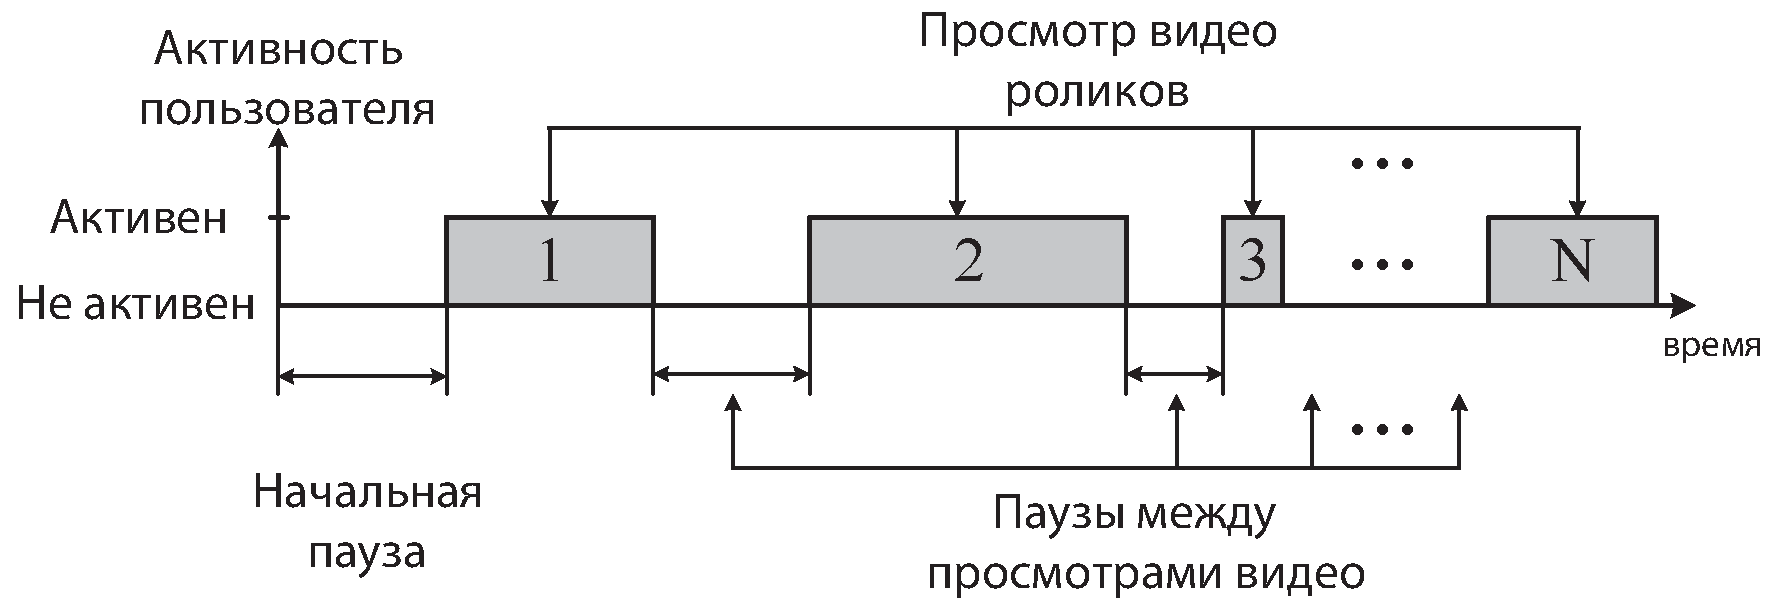
\includegraphics[width=\textwidth]{Chapter1/UserActivity.pdf}
\caption{Модель поведения пользователя при просмотре видео}
\label{fig:UserActivity}
\end{center}
\end{figure}

Описанная выше модель поведения пользователя может быть определена следующим набором случайных величин:
\begin{itemize}
  \item Длительность интервала времени перед заказом первого видео;
  \item Длительность заказанного видеоряда;
  \item Длительность пауз между просмотрами видео.
\end{itemize}

Таким образом, при наблюдении за трафиком, проходящим через сетевой (и нижележащие) уровень семиуровневой модели OSI, фиксируется чередование периодов наличия и отсутствия (пульсации) трафика у абонента. Однако, данное утверждение задает лишь обобщенную модель трафика со стороны пользователя системы передачи видеоданных. Для того чтобы окончательно определить модель генерируемого трафика необходимо рассмотреть аспекты работы видеоплеера в активный период загрузки видеопоследовательности.

В настоящие дни существует огромное множество сервисов хранения видеоданных и каждый из них представляет собственный программный комплекс, обеспечивающий загрузку видео с уникального сервиса. Исходя из данного факта провести обзор всех возможных видеоплееров не представляет возможным, поэтому в данной работе будет представлена обобщенная модель видеоплеера. Данная модель, не теряя общности, описывает все важные аспекты работы всевозможных плееров видеоданных.

На рисунке~\ref{fig:Player_avt} изображен конечный автомат видеоплеера. В начальный момент времени плеер находит в состоянии \textit{Ожидания} начала загрузки, нахождение в данном состоянии обусловлено ожиданием указаний от пользователя. После получения команды пользователя о начале загрузки будет установлено соединение с сервером хранения видеоданных и произведен переход в состояние \textit{Буферизация}.

\begin{figure}[htbp]
\begin{center}
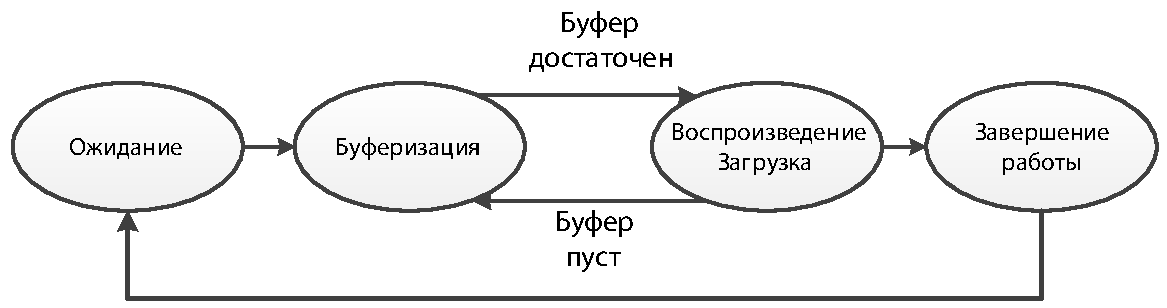
\includegraphics[width=\textwidth,height=0.2\textheight]{Chapter1/player_avt.pdf}
\caption{Конечный автомат видеоплеера}
\label{fig:Player_avt}
\end{center}
\end{figure}

В состоянии \textit{Буферизация} видеоплеер не осуществляет демонстрацию загружаемых видеоданных, а производит накопление видеоданных до определенного уровня для последующей демонстрации. Осуществление буферизации на воспроизводящем устройстве призвано уменьшить негативные эффекты воспроизведения, вызванные изменением свойств канала передачи данных, что особенно актуально для беспроводных систем передачи данных. Пребывание в данном состоянии является негативным эффектом при просмотре видео. После накопления достаточной длительности видеопоследовательности в буфере видеоплеер переходит в состояние \textit{Воспроизведение и Загрузка}.

В течении состояния \textit{Воспроизведение и Загрузка} плеер решает две важные задачи: демонстрация контента и адаптация загружаемого потока для максимизации длительности возможного времени воспроизведения. Вторая задача не является тривиальной и решается, в рассмотренных далее реализациях, эвристическими методами. Важно отметить, что в данном состоянии происходит одновременное наполнение и опустошением буфера на пользовательском устройстве, и если скорость наполнения будет меньше скорости опустошения, то в некоторый момент времени в буфере не найдется необходимого объема данных для обеспечения демонстрации. Описанное событие называется опустошение буфера, и при его наступлении видеоплеер возвращается в состояние \textit{Буферизация}, где будет находиться до накопления достаточного объема видеоданных.

В некоторый момент времени будет закончена загрузка видеоданных на пользовательское устройство. И видеоплеер осуществит переход в состояние \textit{Завершение Работы}. В данном состоянии будет закрыто соединения с сервером и ожидание окончания просмотра, после чего видеоплеер переходит в состояние \textit{Ожидания} начала загрузки.

Завершающим шагом для описания модели генерируемого трафика при просмотре видео является рассмотрение существующих методов адаптации загружаемого потока для максимизации длительности возможного времени воспроизведения в состоянии \textit{Воспроизведения и Загрузки}. Всевозможные плееры видеоданных разделяются на два множества:
\begin{itemize}
  \item HTTP Progressive Download (HPD)~--~множество плееров, не осуществляющих адаптацию видеопотока;
  \item HTTP Adaptive Streaming (HAS)~--~множество плееров, осуществляющих адаптацию видеопотока.
\end{itemize}
Для упрощения терминологии и уменьшения используемых англоязычных аббревиатур далее в работе при обозначении плееров HPD будет использоваться термин \textit{неадаптивные}, а для обозначения плееров HAS~--~\textit{адаптивные}

В начале тысячелетия в сети Интернет все видео были представлены лишь в одной репрезентации, и для их доставки использовались реализации неадаптивных плееров. Однако, даже в настоящее время неадаптивные плееры очень широко распространены. Они используются в браузере Safari для загрузки видеоданных с сервиса YouTube, для просмотра видео в социальной сети Facebook и при передаче трансляций в режиме реального времени (спортивные соревнования, прессконференций и т. д.). Как правило, для мероприятий, транслирующихся в реальном времени, не организуется кодирование видеопотока для нескольких репрезентаций, а доступна лишь одна для ознакомления с содержанием мероприятия.

Далее приведено описание работы неадаптивного плеера в состоянии \textit{Буферизация} и \textit{Воспроизведение и Загрузка}. После получения команды от пользователя о начале загрузки некоторого видео на пользовательское устройство загружается MPD файл с описанием последовательности, и пользователю предлагается выбрать репрезентацию для просмотра. На основе выбранной репрезентации будет отправлен запрос на контент сервер, который организует последовательную отправку сегментов видео на воспроизводящее устройство. Далее происходит буферизация последовательности некоторой длительности и после окончания буферизации начнется воспроизведение. Если по каким-либо причинам пользователь желает изменить репрезентацию просматриваемого видео, то на сервер будет отправлен новый запрос с ее указанием и идентификатором сегмента, с которого необходимо начать передачу видеоданных (рисунок~\ref{fig:hpd_logic}). Логика отправки запросов на контент сервер регламентируется правилом: \textit{<<запрос на новый сегмент отправляется после получения текущего загружаемого сегмента>>}.

\begin{figure}[htbp]
\begin{center}
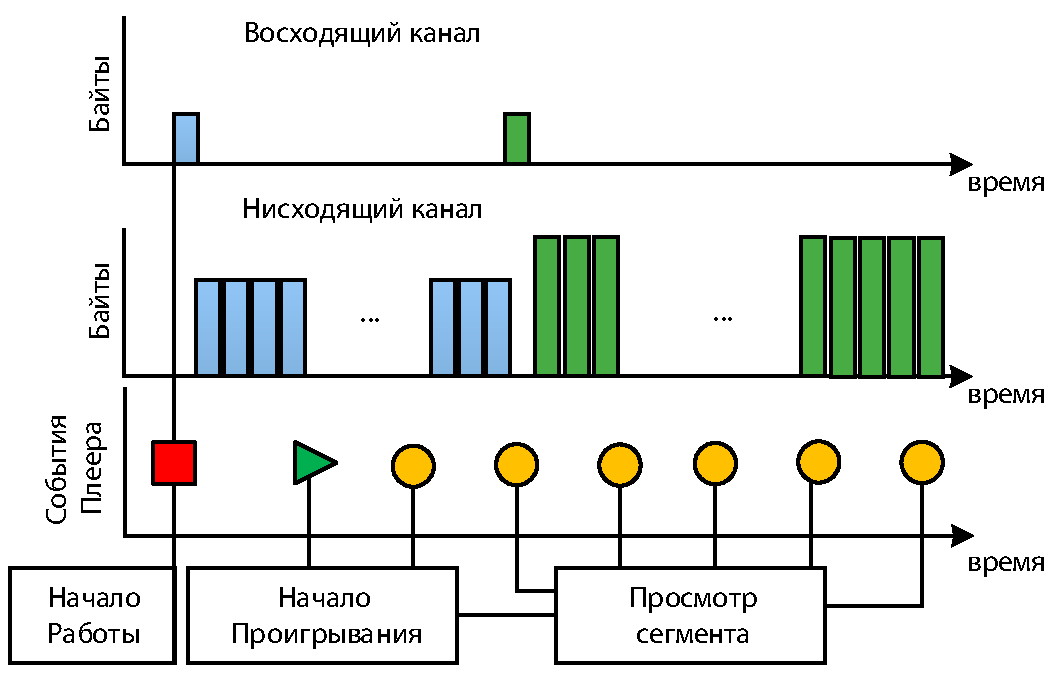
\includegraphics[width=0.7\textwidth]{Chapter1/hpd_logic.pdf}
\caption{Логика работы неадаптивного видеоплеера}
\label{fig:hpd_logic}
\end{center}
\end{figure}

Во время работы неадаптивного видеоплеера в состоянии \textit{Воспроизведение и Загрузка} на сетевом уровне наблюдается постоянный поток видеоданных в нисходящем канале (от видео сервера к пользователю), а в восходящем канале редкие запросы от воспроизводящего устройства.

Таким образом, модель генерируемого трафика при работе неадаптивного видеоплеера представляется последовательностью периодов высокой нагрузки на сеть передачи данных со случайными паузами между ними. Длительность периодов высокой нагрузки определяется только длительностью видео и выбранной репрезентацией, без учета текущей ситуации в сети. Подобная модель модель поведения значительно увеличивает нагрузку на систему передачи данных.

За последние десять лет количество обслуживаемых устройств в сетях передачи данных росло в геометрической прогрессии. И в начале первого десятилетия 21-го века стало очевидно, что существующие телекоммуникационные сети, особенно мобильные, не обладают достаточной емкостью для обеспечения достаточного качества обслуживания большого числа абонентов, одновременно просматривающих видеоконтент. Под емкостью сети понимается максимальное число пользователей, которое может одновременно находится в сети, с необходимым уровнем качества обслуживания каждого активного пользователя. Ввиду невозможности кардинального изменения существующих телекоммуникационных систем для доставки видео был разработан новый стандарт для передачи видеоданных Moving Picture Experts Group Dynamic Adaptive Streaming over HTTP (MPEG-DASH), который позволяет частично решить проблему емкости сети~\cite{dash_standard}. В настоящее время представлена версия стандарта 3GP-DASH в спецификации консорциума, разрабатывающего решения для беспроводной связи 3GPP \cite{conviva}. Стандарт 3GP-DASH включает в себя описание адаптивной и неадаптивной технологии передачи видео по протоколу HTTP.

Стандарт DASH описывает лишь формат представления видеоданных (подраздел~\ref{chap1:VideoFormat}) и общие идеи правил формирования запросов видеоплеера к серверу на сегменты видео, которые позволяют организовать адаптивную передачу видеопотока для специфичных требований каждого конкретного сервиса доставки контента. Обобщенная логика работы видеоплеера, описывающая основную идею представленную в стандарте DASH, демонстрирует рисунок~\ref{fig:has_logic}.

\begin{figure}[htbp]
\begin{center}
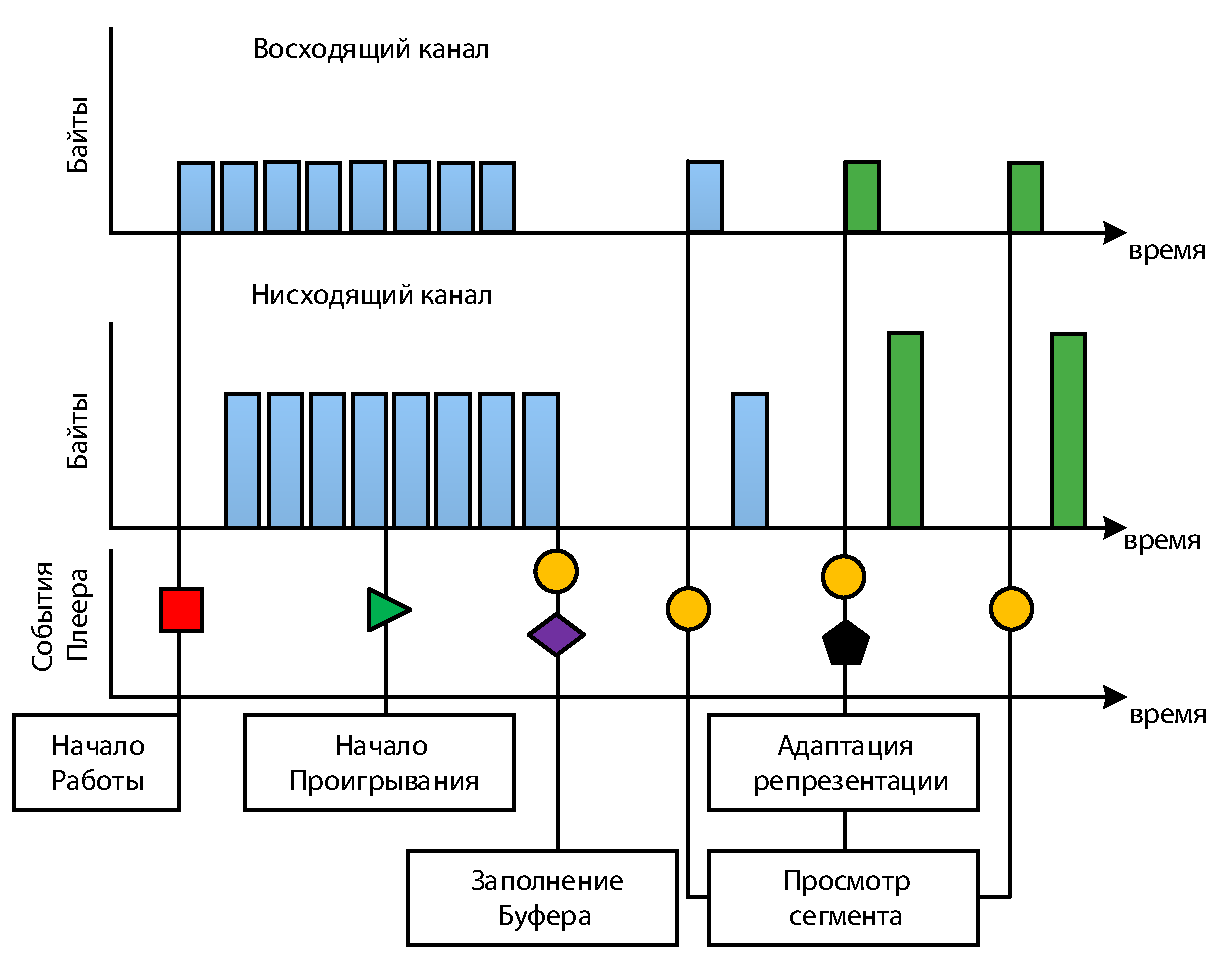
\includegraphics[width=0.7\textwidth]{Chapter1/has_logic.pdf}
\caption{Логика работы адаптивного видеоплеера}
\label{fig:has_logic}
\end{center}
\end{figure}

После установки соединения с контент сервером и загрузки MPD файла видеоплеер самостоятельно генерирует и отправляет первый запрос на видеоданные. После загрузки каждого сегмента производится оценка скорости получения данных и длительности загруженного видео, на основе которых механизм адаптации видеоряда выберет репрезентацию для следующего сегмента. В состоянии \textit{Воспроизведение и Загрузка} изменяется логика отправки запросов на сегменты данных с \textit{<<запрос на новый сегмент отправляется после \textbf{получения текущего загружаемого сегмента}>>} на \textit{<<запрос на новый сегмент отправляется после \textbf{просмотра текущего сегмента}>>}, что приводит к появлению пауз между загрузками сегментов. Наличие алгоритма изменения репрезентации и пауз между загрузками сегментов приводит к уменьшению нагрузки на телекоммуникационные сети, и, как следствие, увеличению их емкости.

Таким образом, важными отличительными особенностями адаптивного видеоплеера от неадаптивного являются:
\begin{itemize}
  \item Отправка плеером запросов на контент сервер для каждого уникального сегмента видеопоследовательности;
  \item Наличие пауз между заказами сегментов в состоянии \textit{Воспроизведение и Загрузка};
  \item Наличие алгоритма адаптации репрезентации под характеристики сети передачи данных.
\end{itemize}

Наибольший интерес из перечисленных выше особенностей представляет алгоритм адаптации репрезентации, так как он имеет непосредственное влияние на модель генерируемого трафика. Как было сказано ранее стандарт DASH не регламентирует данный алгоритм. Однако, существует реализация опорного видеоплеера, который полностью соответствует стандарту DASH. Настоящая реализация была представленна консорциумом DASH Industry Forum, который занимается продвижением настоящего стандарта и предоставляет открытую реализацию видеоплеера и серверных приложений. Данный плеер был реализован в проекте Dash.js, исходный код которого доступен на платформе разработчиков программного обеспечения GitHub~\cite{DashJS}. Плеер Dash.js полностью соответствует требованиям стандарта DASH, постоянно обновляется и дополняется при консультациях с группой экспертов, разрабатывающий данный стандарт. Далее в работе будет описана работа опорного плеера Dash.js версии 1.5. В ходе проведения исследования был проанализирован исходный код на языке JavaScript и проведен комплекс испытаний для подтверждения полученных в ходе анализа исходного кода.

Для наглядного представления результатов проведенного анализа был создан рисунок~\ref{fig:abr}, описывающий логику адаптации битовой репрезентации видеоплеером в состояниях \textit{Буферизация} и \textit{Воспроизведение и Загрузка}. Все решения алгоритма адаптации репрезентации основаны на значении параметра \textit{<<Уровень Буфера>>}~--~длительность загруженной видеопоследовательности на пользовательском устройстве в секундах, доступной для воспроизведения. Например, при значении \textit{<<Уровень Буфера>>} равном 5-ти секундам на воспроизводящем устройстве доступно к воспроизведению 5 секунд видео в текущий момент времени, и если плеер находится в состоянии \textit{Воспроизведение и Загрузка} и в течение 5-ти секунд не будет загружен ни один сегмент, то воспроизведение прекратится и плеер перейдет в состояние \textit{Буферизация}.

Плеер Dash.js является многопоточным приложением и его работа организована в трех основных потоках, одновременно исполняющихся на пользовательском устройстве: ПРОИГРЫВАНИЕ, ЗАГРУЗКА и МОНИТОРИНГ.

В начальный момент времени работы плеера доступен MPD файл с описанием каждого сегмента видеопоследовательности, и необходимо решить задачу выбора репрезентации для первого сегмента видеопоследовательности. Для решения данной задачи реализована функция подбора репрезентации по оценке скорости получения данных. Словесно данная функция может быть описана следующим образом: найти ближайшую снизу репрезентацию с битовой скоростью не превышающую оценку скорости. Она вызывается в блоках, где присутствует команда <<Запросить>>. Для первого сегмента будет подобрана репрезентация ближайшая к скорости 1 Мбит/с, отправлен запрос на сервер и запущен поток приема данных~--~ЗАГРУЗКА.

\begin{landscape}
\begin{figure}[h]
\begin{center}
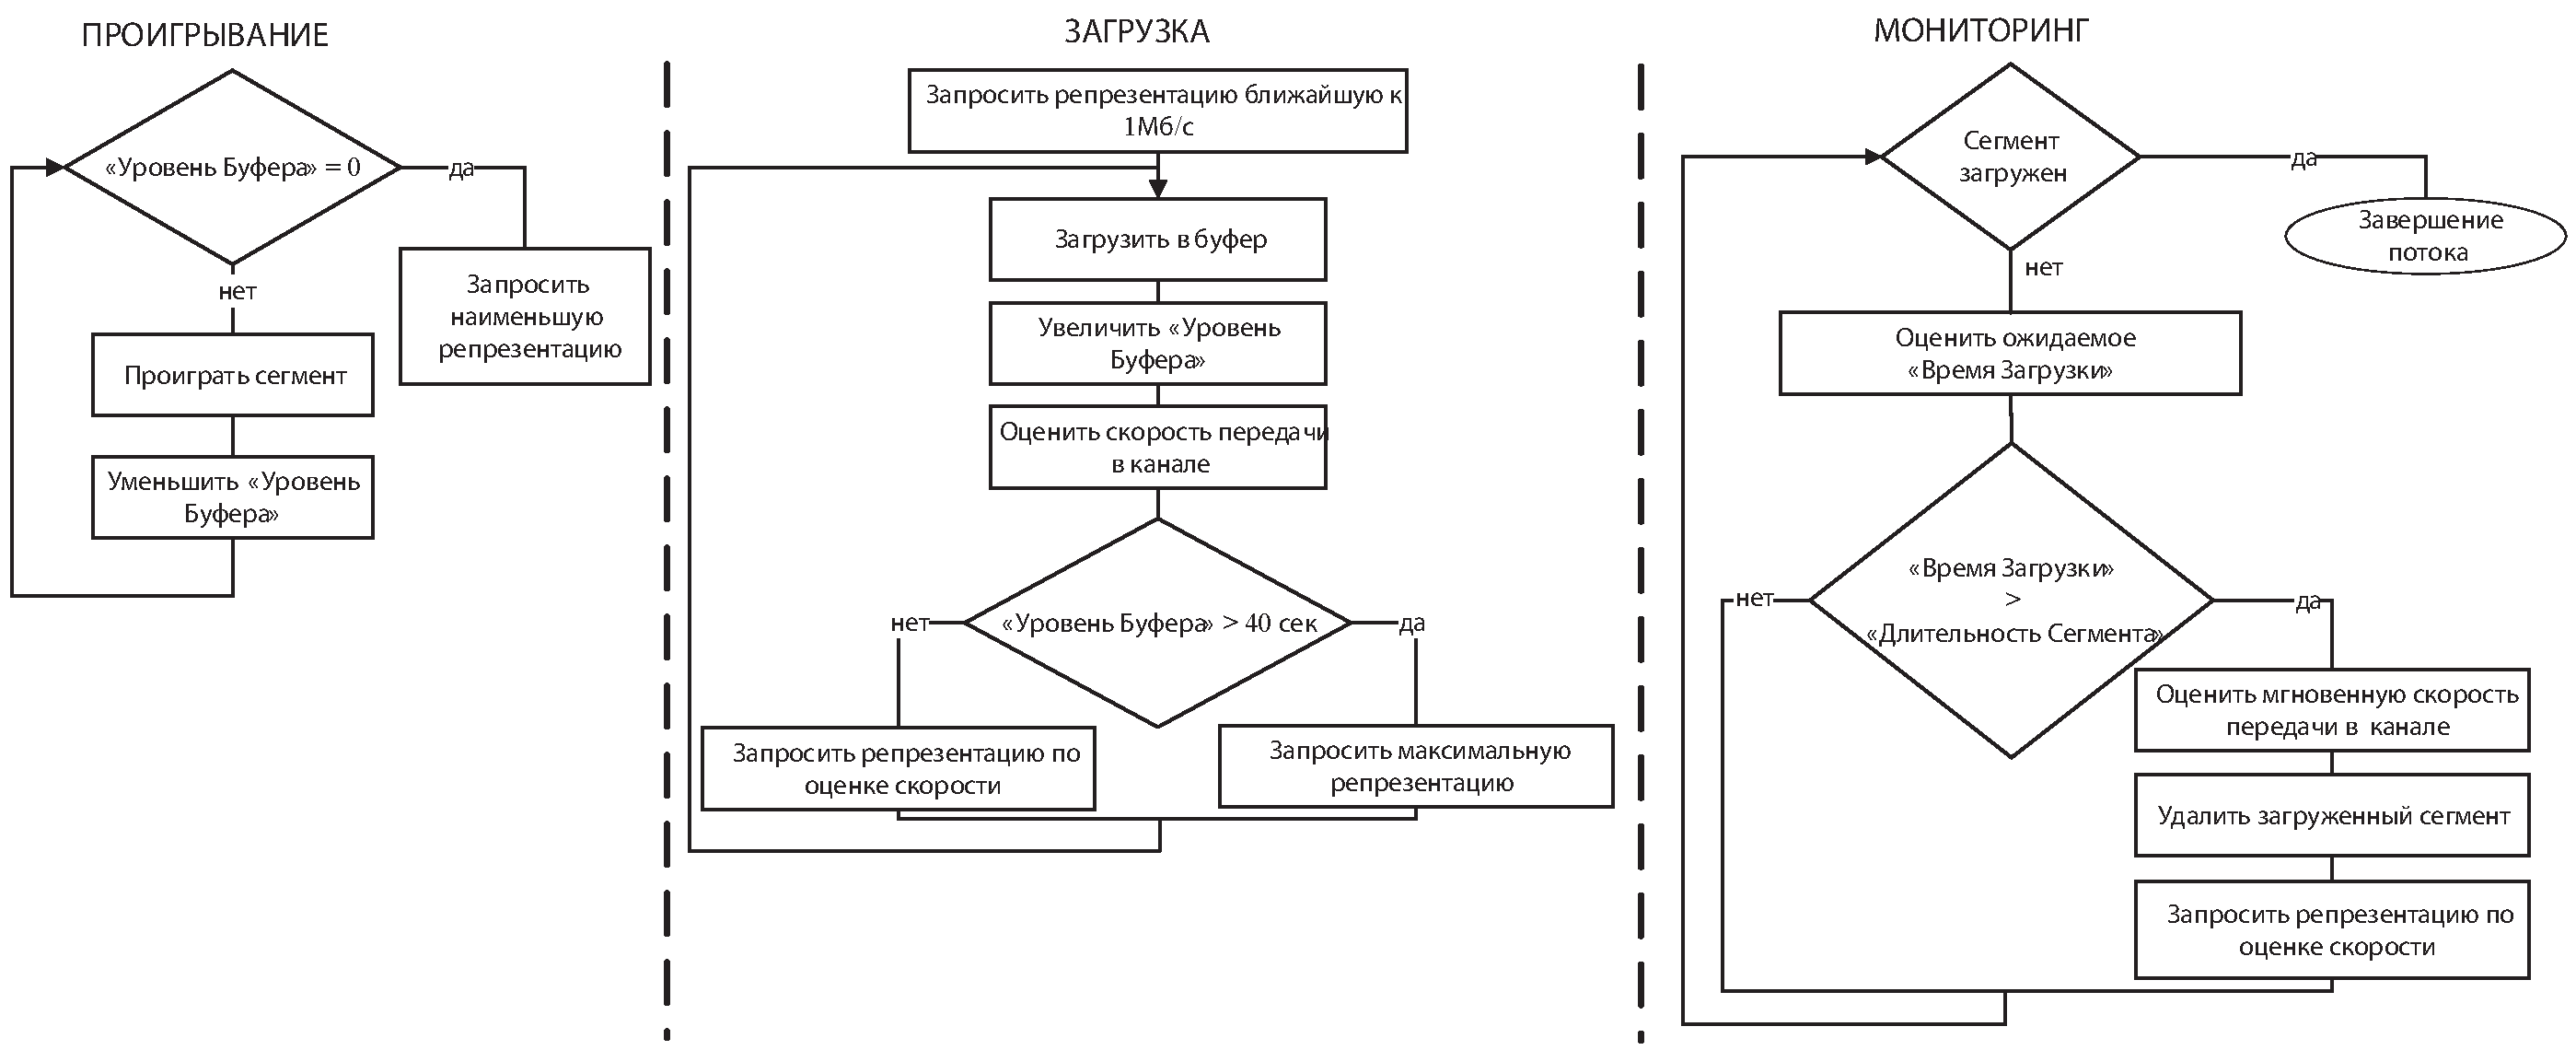
\includegraphics[width=1.5\textwidth,height=0.7\textheight]{Chapter1/abr.pdf}
\caption{Логика адаптации репрезентации опорного видеоплеера Dash.js}
\label{fig:abr}
\end{center}
\end{figure}
\end{landscape}

В потоке ЗАГРУЗКА происходит прием данных с нижележащих уровней сети, формирование сегментов видеопоследовательности и помещение их в буфер на воспроизводящем устройстве. Рассмотрим цикл загрузки одного сегмента видео. После отправки запроса на сервер в нисходящем канале начинается передача данных, и необходимо организовать их прием, контроль корректности, порядка и полноты загрузки данных. Когда сегмент будет полностью доставлен на воспроизводящее устройство он будет загружен в буфер, и значение параметра \textit{<<Уровень Буфера>>} увеличено на длительность загруженного сегмента. Далее для выбора репрезентации для следующего сегмента производится оценка скорости загрузки данных в два этапа:
\begin{enumerate}
  \item Вычисление оценки скорости загрузки текущего сегмента, как отношение размера сегмента к длительности его загрузки;
  \item Вычисление результирующей оценки скорости загрузки как среднего арифметического оценок скоростей нескольких последних сегментов и умножение полученного значения на понижающий коэффициент. Занижение результирующего значения необходимо для компенсации возможных колебаний скорости загрузки данных.
\end{enumerate}
Далее значение параметра \textit{<<Уровень Буфера>>} сравнивается с порогом достаточного уровня буфера. Если значение \textit{<<Уровень Буфера>>} выше, то следущий сегмент будет заказан в максимальной доступной репрезентации, иначе выбор репрезентации будет основан на вычисленной ранее оценке.

Одновременно с потоком ЗАГРУЗКА работает поток МОНИТОРИНГ, задачей которого является контроль длительности загрузки сегментов. Для этого в каждый момент времени загрузки происходит оценка ожидаемого времени загрузки сегмента и если данная оценка превышает произведение длительности сегмента и коэффициента порогового ожидания загрузки, то загрузка текущего сегмента будет прекращена. При прекращении загрузки все загруженные данные удаляются и в этот же момент, сервер уведомляется о прекращении загрузки сегмента и на него отправляется новый запрос с указанием репрезентации, выбранной на основе оценки скорости загрузки только текущего сегмента.

После накопления размера достаточной для начала воспроизведения длительности видео будет запущен поток ПРОИГРЫВАНИЕ, который производит демонстрацию загруженного в буфер видео. При проигрывании сегмента он изымается из буфера, и значение \textit{<<Уровень Буфера>>} уменьшается на длительность, изъятого сегмента. Данный поток влияет на выбор репрезентации только в том случае, когда уровень буфера равен нулю (в буфере нет данных для воспроизведения), тогда плеер прекращает демонстрацию видео, переходит в состояние \textit{Буферизация}, а следующий сегмент будет заказан в минимальной репрезентации.

На представленный выше алгоритм адаптации видеоряда под условия канала передачи данных налагается ограничение на частоту переключения репрезентаций видео. Очевидным является факт, что частое переключение битовых репрезентаций негативно влияет на качество восприятия видеопотока: в некоторых случаях быстрое переключение репрезентаций при просмотре приводит к проявлению симптомов неврологических расстройств. Поэтому в современных реализациях видеоплееров количество переключений в единицу времени ограничено сверху~\cite{widash}.

Основные параметры видеоплеера Dash.js были агрегированы в таблице~\ref{tab:DashJSParams}.

\begin{table}[!h]
    \caption{Основные параметры адаптивного видеоплеера Dash.js}
    \begin{center}
		\label{tab:DashJSParams}
	    \begin{tabular}{| C{4cm} | C{7cm} | C{3cm} |}
	    	\hline
	    	Название параметра & Описание & Значение \\
	    	\hline
	    	\multicolumn{3}{|c|}{Общие параметры} \\
	    	\hline
	    	Длительность сегмента видеоданных & Длительность сегментов, на которые разделена видеопоследовательность & [2, 10] секунд \\
	    	\hline
	    	Размер начальной буферизации & Длительность видеопоследовательности, которая должна быть загружена перед началом воспроизведения & 12 секунд \\
	    	\hline
	    	Максимальный размер буфера & Максимальная длительность видеопоследовательности, которая может быть помещена в буфер & 60 секунд \\
	    	\hline
	    	\multicolumn{3}{|c|}{Параметры адаптации репрезентации} \\
	    	\hline
	    	Начальная оценка канала & Оценка канала передачи данных, на основе которой будет выбрана репрезентация первого сегмента & 1 Мбит/c \\
	    	\hline
	    	<<Память>> при оценке скорости канала & Число сегментов, на основе которых будет производиться оценка скорости канала передачи данных & 3 \\
	    	\hline
	    	Понижающий коэффициент оценки скорости & Коэффициент для понижения оценки скорости передачи данных, при оценке скорости загрузки & 0.9 \\
	    	\hline
	    	Достаточный уровень буфера & Длительность буферизированного видеопотока, при котором плеер будет заказывать только максимальную репрезентацию & 40 секунд \\
	    	\hline
	    	Коэффициент порогового ожидания загрузки сегмента & Длительность числа сегментов, которых будет ожидать плеер, перед удалением текущего сегмента & 1.5 \\
	    	\hline
    	\end{tabular}
	\end{center}
\end{table}

Для адаптивного видеоплеера модель генерируемого трафика зависит как от характеристик просматриваемого видеопотока, так и системы передачи данных. Она определяется настройками видеоплеера и алгоритма адаптации репрезентации.

На текущий момент был представлен анализ организации передачи видео в телекоммуникационных сетях. Рассмотрены основные виды видеоплееров и показано влияние плеера на модель генерируемого трафика. Исходя из проведенного анализа возможно заключить, что обслуживание передачи видеоданных является нетривиальной задачей. Наиболее важным для исследования становится вопрос о влиянии характеристик сети передачи данных и видеоплеера на качество обслуживания абонента. Именно данному вопросу посвящена следующая часть раздела.

\section{Методики оценки качества передачи видеоконтента}
\label{chap1:VideoMOS}

Оценка качества передачи видеоконтента является сложной задачей ввиду субъективного восприятия пользователем характеристик воспроизведения. Существуют два основных подхода для оценки качества для всевозможных сервисов:
\begin{itemize}
  \item Экспертная оценка~\cite{Experts};
  \item Оценка пользовательского опыта использования сервиса~\cite{QoE}.
\end{itemize}

Изначально для определения качества телекоммуникационных сервисов использовались экспертные оценки. Получение подобной оценки состояло из нескольких этапов: подбор членов экспертной комиссии, формулировка строго поставленных вопросов и ожидание результата. Данная процедура занимает много времени, как следствие, использование экспертной оценки имеет смысл только уже к разработанным системам передачи данных, однако для оценки качества на этапе разработки системы использовать данный подход не представляется возможным. В настоящее время мнения экспертов используют для формирования требований к разрабатываемым стандартам связи следующего поколения.

В тоже время, наличие положительной экспертной оценки не является гарантией удовлетворенности пользователя использованием сервисом. Данный факт привел к появлению второго метода оценки качества: оценка пользовательского опыта использования сервиса, в англоязычной литературе этот термин известен как Quality of Experience (QoE). Термин QoE очень общий и включает в себя огромное число методик и критериев для различных сервисов, любой критерий с системой сравнения результатов, отражающий пользовательский опыт, считается QoE.

Для оценки качества телекоммуникационных сервисов была принята методология оценки, известная как Mean Opinion Score (MOS)~\cite{MOS_termin}. Результат оценки MOS представляется числом в отрезке от одного до пяти, где единица описывает наименьшую степень удовлетворенности пользователя, а пять наивысшую. Считается, что пользователь удовлетворен качеством сервиса, если значение MOS больше или равно трем. Для получения оценки MOS собирается статистически оправданная группа пользователей, с учетом расового, полового, возрастного и т.д. факторов, производится демонстрация сервиса, и на ее основе члены группы выставляют оценки. Результирующее значение выражается как среднее арифметическое всех даных оценок. Описанный выше путь получения оценки обладает такими же недостатками, как и экспертная оценка, однако полученный результат является более показательным, и на его основе можно организовать сравнение систем связи.

Множество усилий было направлено на ускорение получения оценки восприятия качества обслуживания, и в настоящее время для каждого вида сервисов существуют разработанные рекомендации по вычислению значения MOS. В каждой подобной рекомендации присутствует описание методологии, которая на основе огромного массива объективных характеристик доступных на пользовательском устройстве вычисляет значение оценки. Полученное значение, по утверждению авторов, не отличается от оценки, поставленной опрашиваемыми пользователями. Важно отметить следующий факт: применимость различных методологий оценки качества восприятия ограничивается типом используемого видеоплеера, например, существуют методологии, которые могут вычислить достоверное значение оценки только если при демонстрации использовался неадаптивный видеоплеер.

Организацией International Telecommunication Union, известной в РФ как Международный Союз Электросвязи, была стандартизирована процедура вычисления MOS для видеопоследовательностей с неизменяемой репрезентацией длительностью от 30-ти до 60-ти секунд~\cite{VIDEO_MOS}. Ввиду большого объема методологии, описанной в~\cite{VIDEO_MOS}, в данной работе будет представлено лишь ее описание на качественном уровне. Далее в работе для сокращения длины названий в качестве обозначения данной методологии будет называться термин ITU MOS.

Изначально на основе объективных характеристик рассчитываются два основных фактора при просмотре видео:
фактор качества видео и фактор воспроизведения~(рисунок~\ref{fig:MOS_diag}). Фактор качества видео оценивает восприятие пользователем характеристик неискаженного видеопотока на конкретном воспроизводящем устройстве. В качестве входных параметров данный фактор учитывает разрешение экрана воспроизводящего устройства, битовую скорость, частоту кадров и настройки кодирования видео и аудио потоков. Наличие, в приведенном выше списке, настроек видеокодека обусловлено влиянием алгоритма сжатия на потерю качества видеоданных. На выходе возвращается значение, нормированное в отрезке от 1-цы до 5-ти.

\begin{figure}[htbp]
\begin{center}
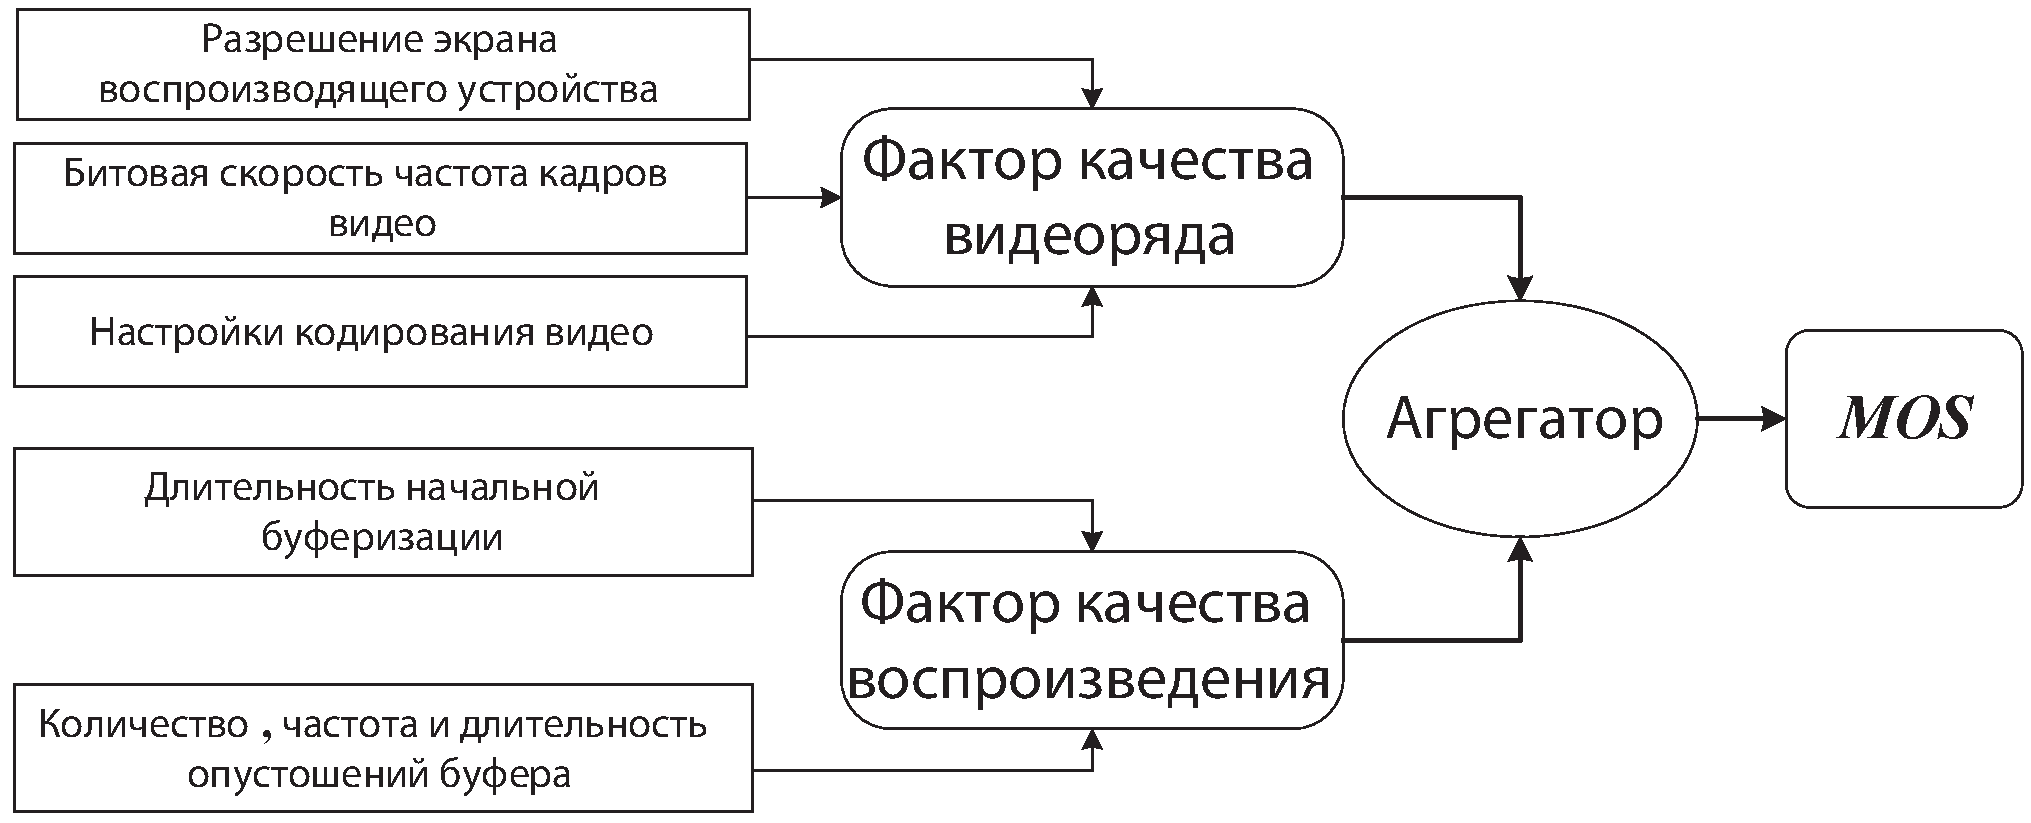
\includegraphics[width=\textwidth]{Chapter1/MOS_diag.pdf}
\caption{Схема вычисления оценки качества передачи видео в методологии ITU MOS}
\label{fig:MOS_diag}
\end{center}
\end{figure}

Фактор воспроизведения оценивает восприятие пользователем характеристик воспроизведения. Выделяются два основных негативных эффекта, имеющих определяющее влияние на оценку пользователем воспроизведение видео: начальная буферизация и опустошение буфера. Начальная буферизация характеризуется длительностью интервала времени от получения от пользователя команды о запросе видео до начала демонстрации загруженных данных (длительность нахождения в состоянии \textit{Буферизация} в начале работы видеоплеера). Считается, если длительность начальной буферизации превышает некторое значение, то пользователь откажется от просмотра.

Второй негативный эффект воспроизведения видео~--~опустошение буфера. Он характеризуется событием перехода видеоплеера из состояния \textit{Воспроизведение и Загрузка} в состояние \textit{Буферизация}, ввиду недостатка видеоданных загруженных в буфер воспроизводящего устройства. Наиболее важными в методологии ITU MOS считаются моменты времени переходов из состояний, длительности повторного нахождения в состоянии \textit{Буферизация} после осуществления начальной буферизации. Из моментов времени переходов рассчитывается частота опустошений буфера при воспроизведении видео. В методологии ITU MOS наличие хотя бы одного опустошения критично снижает оценку качества воспроизведения. На выходе фактора воспроизведения так же представляется числом от 1-цы до 5-ти.

Важным моментом работы методологии ITU MOS является метод агрегации представленных выше факторов, определяемый следующим выражением:
$$ITU MOS = max ([VideoQualityFactor - 5 + VideoPlayingFactor], 1 ),$$
где $VideoQualityFactor$~--~фактор качества видео и $VideoPlayingFactor$~--~фактор воспроизведения.

Из вида данного выражения следует, что результирующее значение MOS не может превышать оценки фактора качества видео: при идеальном воспроизведении (оценка фактора воспроизведения равна 5-ти) результирующее значение равно оценке фактора качества видео, а любое уменьшение качество воспроизведения уменьшает результат.

Основным недостатком методологии ITU MOS является его ограниченная сфера применимости, так как она может быть использована для видеопоследовательностей с неизменной битовой скоростью (неадаптивный видеоплеер) и длительностью не превышающих 60-ти секунд. Также реализация данной методологии затруднено ввиду использования огромного объема информации для вычисления оценки. В работе методология ITU MOS приведена в качестве опорного метода оценки качества восприятия видеоряда, так как все остальные методологии основаны на данной.

В настоящее время предложено несколько методологий оценки качества восприятия просмотра видео. Ярким представителем таких методологий является решение компании Huawei под названием U-vMOS (User, Unified, Ubiquitous-Mean Opinion Score for Video), которая ставит перед собой задачу оценки качества видео без ограничений на их длительность и изменение битовых скоростей. Методология Huawei U-vMOS была представлена в апреле 2016-го года на выставке London TV Connect Exhibition~\cite{UvMOSWhitePaper}.

Подробное описание данной методологии представлено в презентации на сайте компании~\cite{UvMOSPresentation}. В отличии от методологии ITU MOS, для расчета значения U-vMOS требуется намного меньшее число параметров.

Для расчета результирующей оценки качества восприятия видео по методологии U-vMOS должны быть оценены три фактора для одного сегмента видео:
\begin{itemize}
  \item Фактор качества видеоданных (sQuality);
  \item Фактор ожидания начала проигрывания (sItreraction);
  \item Фактор качества воспроизведения (sView).
\end{itemize}
Далее, для обозначения представленных факторов, будут использоваться оригинальные англоязычные термины.

Фактор sQuality описывает восприятие пользователем просмотра видеоряда некоторого разрешения на типовом экране воспроизводящего устройства. Авторами методологии U-vMOS, в качестве типовых экранов, были рассмотрены экран телевизионного устройства (42 дюйма) и экран смартфона (5.5 дюйма). Значение sQuality задано таблицой~\ref{tab:sQuality}.

\begin{table}[!h]
    \caption{Фактор качества видеоданных (sQuality) в методологии U-vMOS}
    \begin{center}
		\label{tab:sQuality}
	    \begin{tabular}{|c|c|c|}
		\hline
		\multirow{2}{*}{Разрешение} & \multicolumn{2}{c|}{Оценка} \\
		 & \multicolumn{2}{c|}{sQuality} \\
		\cline{2-3}
		репрезентации & Телевизионный & Экран\\
		 & экран & сматрфона\\
		\hline
		2880p (5K) & 4.78 & 5 \\
		\hline
		2160p (4К) & 4.65 & 4.78 \\
		\hline
		1440p (2К) & 4.2 & 4.58 \\
		\hline
		1080p (Full HD) & 4 & 4.45 \\
		\hline
		720p (HD) & 3.15 & 4 \\
		\hline
		480p & 2.44 & 3.64 \\
		\hline
		360p & 1.66 & 3 \\
		\hline
		\end{tabular}
	\end{center}
\end{table}

Фактор sInteraction описывает удовлетворенность пользователем длительностью ожидания в секундах начала воспроизведения потока и задается таблицей~\ref{tab:sIteraction}. Данная оценка является общей для всех сегментов видео и вычисляется только для первого сегмента.

\begin{table}[!h]
    \caption{Фактор ожидания начала воспроизведения (sInteraction) в методологии U-vMOS}
    \begin{center}
		\label{tab:sIteraction}
	    \begin{tabular}{| C{4cm} | C{5cm} | C{4cm} |}
	    	\hline
	    	Оценка sInteraction & \multicolumn{2}{c|}{Длительность начальной буферизации}\\
	    	\cline{2-3}
	    	& Телевизионный экран & Экран смартфона \\
	    	\hline
	    	5 & < 100 мс & < 100 мс \\
	    	\hline
			4 & 1 сек & 1 сек \\
	    	\hline
			3 & 2 сек & 3 сек \\
	    	\hline
			2 & 5 сек & 5 сек \\
	    	\hline
			1 & $\geq$ 8 сек & $\geq$ 10 сек \\
	    	\hline
    	\end{tabular}
	\end{center}
\end{table}

Важным фактором воспроизведения является sView. В качестве оцениваемой характеристики используется процент времени ожидания возобновления просмотра после события опустошения буфера к длительности сегмента видео. Оценка качества воспроизведения так же является таблично заданной функцией (таблица~\ref{tab:sView}).

\begin{table}[!h]
    \caption{Фактор качества воспроизведения (sView) в методологии U-vMOS}
    \begin{center}
		\label{tab:sView}
	    \begin{tabular}{| C{4cm} | C{5cm} | C{4cm} |}
	    	\hline
	    	Оценка sView & \multicolumn{2}{|c|}{Процент времени прерывания воспроизведения}\\
	    	\cline{2-3}
	    	& Телевизионный экран & Экран смартфона \\
	    	\hline
			5 & 0\% & 0\%\\
	    	\hline
			4 & 0.1\% & 5\%\\
	    	\hline
			3 & 1\% & 10\%\\
	    	\hline
			2 & 5\% & 15\%\\
	    	\hline
			1 & $\geq$ 10\% & $\geq$ 30\%\\
	    	\hline
    	\end{tabular}
	\end{center}
\end{table}

После того как были рассчитаны все вышеперечисленные показатели качества результирующее значение для одного сегмента может быть получено следующим образом:
$$UvMOS = (sQuality - 1)\left[\frac{\alpha(sInteraction - 1)+\beta(sView-1)}{4(\alpha+\beta)}\right] + 1,$$
где коэффициенты $\alpha$ и $\beta$ заданы таблицей~\ref{tab:Cofficients}.

\begin{table}[!h]
    \caption{Коэффициенты для расчета значение MOS в методологии U-vMOS}
    \begin{center}
		\label{tab:Cofficients}
	    \begin{tabular}{| C{4cm} | C{4cm} | C{4cm} |}
	    	\hline
	    	Коэффициент & Телевизионный экран & Экран смартфона \\
	    	\hline
			$\alpha$ & 0.66 & 0.71\\
	    	\hline
			$\beta$ & 0.77 & 0.77\\
	    	\hline
    	\end{tabular}
	\end{center}
\end{table}

Из вида функции U-vMOS следует, что если зафиксировать некоторое значение показателя sQuality, то результирующее значение не может превышать значение данного показателя. Таким образом, чтобы получить значение MOS превышающее 3, то необходимо демонстрировать пользователю видеопоток с разрешением не менее 720p и 360p для телеэкранов и смартфонов соответственно. Показатели качества sInteraction и sView, отличные от 5-ти только понижают результирующее значение MOS. Как следствие, для обеспечения значения U-vMOS больше трех следует обеспечивать более высокие репрезентации.

Компанией Huawei был представлен программный комплекс для разработчиков систем, который позволяет оценить качество воспроизведения на стороне пользовательского устройства для большинства платформ~\cite{UvMOSSdk}. Реализованный программный комплекс представлен в виде библиотеки на языке С++. Он позволяет оценить качество для адаптивного видеопотока неограниченной длительности, на основе методики U-vMOS. На вход поступают <<сырые>> данные для каждого просмотренного сегмента: разрешение, битовая скорость, прерывание воспроизведения и длительность ожидания начала воспроизведения. На выходе представлены оценки воспроизведения потока (sQuality, sInteraction, sView) и результирующее значение оценки удовлетворенности пользователя от просмотра.

Таким образом, метод оценки Huawei U-vMOS применим для адаптивного и неадаптивного видеопотока. Данное свойство позволяет использовать его для большего множества видеоконтента, по сравнению со стандартом ITU MOS. Из описания методик оценок качества воспроизведения видео ITU MOS и Huawei U-vMOS, следует что для их использования необходимо иметь доступ к информации на видеоплеере. Данное ограничение значительным образом сужает возможную сферу их применения.

Существует ряд работ, в которых ставится задача анализа и увеличения производительности существующих беспроводных систем при передаче видео, посредствам аналитического исследования функции MOS. Авторы данных работ отмечают, что описанные выше методы невозможно использовать в качестве целевых функций, ввиду большого числа параметров и их сложной, нелинейной взаимосвязи. В подобных работах рассматриваются аппроксимации MOS, которые опираются на меньшее число параметров. Так же утверждается, что оптимизация (минимизация или максимизация) таких аппроксимаций приводит к максимизации функции MOS. В таблице~\ref{tab:appraximations}~(приложение~\ref{AppA}) представлены некоторые аппроксимации, отсортированные в порядке возрастания количества используемых критериев для оценки качества обслуживания.

Таблицу~\ref{tab:appraximations} возможно использовать следующим образом: зафиксировать некоторый объем данных, доступный разработчику сети, и выбрать те критерии качества обслуживания, которые могут оценить удовлетворенность пользователя. Например, при знании битовой скорости просматриваемого потока можно использовать метод, описанный в работе~\cite{Suai2015}, однако, если добавить информацию о длительности опустошения буфера и просмотра возможна более точная оценка на основе критерия~\cite{Essaili_Rate}.

Из результатов, представленных таблицой \ref{tab:appraximations}, были сделаны следующие выводы. На удовлетворенность пользователя просмотром видео влияют два основных фактора:
\begin{itemize}
	\item Фактор качества воспроизводимого потока, определяемый разрешением и частотой кадров. На настоящий фактор оказывает непосредственное влияние битовая скорость потока (таблица \ref{tab:youtubeBr}).
	\item Фактор длительности ожидания (буферизации) в течении просмотра видеопотока.
\end{itemize}
Фактор качества воспроизводимого видео оказывает влияние на удовлетворенность пользователей, использующих адаптивную технологию передачи видеоданных, так как при использовании неадаптивной технологии качество видео выбирается самим пользователем. В свою очередь, фактор длительности ожидания в течении просмотра оказывает влияние на удовлетворенность пользователя вне зависимости от технологии передачи видео (адаптивной и неадаптивной).

Известны два критерия оценки фактора длительности ожидания, представленных в таблице \ref{tab:appraximations}:
\begin{itemize}
	\item \textit{Нормированное отношение длительностей буферизации и просмотра} \cite{QoE_Ozgur,past_tur}:
	\begin{equation}
    	\label{eq:g_def}
    	g_i = \lim\limits_{T\rightarrow\infty} \frac{b_i^T}{w_i^T + b_i^T},
    \end{equation}
    где $b_i^T$~--~общая длительность буферизации пользователя $i$ за время $T$, $w_i^T$~--~общая длительность просмотренного видео пользователем $i$ за время $T$,
	\item \textit{Отношение длительностей буферизации и просмотра} \cite{Bakin_Globecom}:
	\begin{equation}
    	\label{eq:q_def}
    	q_i = \lim\limits_{T\rightarrow\infty} \frac{b_i^T}{w_i^T}.
    \end{equation}
\end{itemize}
В настоящее время, широко исследована производительность беспроводных систем при использовании неадаптивной технологии для критерия качества (\ref{eq:q_def}), однако, для критерия (\ref{eq:g_def}) отсутствуют исследования производительности беспроводных систем связи для передачи видео по протоколу HTTP.

В последующих разделах настоящего диссертационного исследования проводится анализ производительности беспроводной системы связи для критерия качества (\ref{eq:g_def}) при использовании неадаптивной технологии передачи видео, и критерия качества (\ref{eq:q_def}) при адаптивной технологии передачи видеоданных.

После осуществления обзора различных методик оценки качества восприятия видео остается важный вопрос о взаимосвязи объективных показателей производительности сети передачи видеоданных и оценки качества восприятия (подраздел~\ref{chap1:VideoMOS}). Данному вопросу посвящена заключительная часть раздела.

\section{О взаимосвязи объективных показателей производительности сети и оценки качества восприятия видео}
\label{chap1:InterrelationKPIandQoE}

При передаче видеоданных к телекоммуникационной сети предъявляются специфичные требования, обусловленные характеристиками видеоконтента и настройками воспроизводящего устройства. Для разработчиков сетевого оборудования важно обеспечить максимально возможную емкость сети передачи данных, что ставит задачу оценки качества восприятия контента пользователем на основе некоторого объема информации. При разработке или модернизации сетей передачи данных разработчикам доступен ограниченный набор показателей качества обслуживания, который может быть с достаточной точностью оценен на физическом, канальном, сетевом и транспортном уровнях. Однако, показатели работы воспроизводящего устройства, которые имеют наибольшее влияние на удовлетворенность пользователя при просмотре видео, недоступны ввиду шифрования трафика, что делает невозможным получение данной информации на нижележащих уровнях сети.

Вопрос о взаимосвязи характеристик сети и качества обслуживания абонентов прорабатывался в большом количестве работ. Авторы подобных работ представляют список объективных характеристик (в англоязычной литературе обозначается как Key Performance Indicators или сокращенно KPI) сети и указывают их значения, для того чтобы пользователь был удовлетворен качеством обслуживания. В настоящее время современные телекоммуникационные сети и воспроизводящие устройства бурно развиваются, приведенные в данных работах количественные значения показателей изменяются в зависимости от момента написания работ. Однако, список объективных показателей качества обслуживания видеотрафика был неизменным.

На основе анализа работ~\cite{Chen,Cacheda2007,HuaweiReport} был выделен следующий список объективных показателей качества обслуживания пользователя, имеющих наибольшее влияние на передачу видео:
\begin{itemize}
  \item \textit{Задержка}~--~интервал времени от момента отправки пакета передающей стороной и до момента получения подтверждения от приемной стороны о получении пакета. В англоязычной литературе для обозначения данного вида задержки используется термин \textit{Round Trip Time}, в русскоязычной двусторонняя.

  В реальной системе задержка является случайной величиной. Как следствие, во всех работах в качестве количественного показателя приводится оценка математического ожидания данной случайной величины. Кроме математического ожидания задержку так же характеризуют параметром, который в англоязычной литературе называют Packet Delay Variation~\cite{Jitter}. Достаточно часто как в русскоязычной, так и англоязычной литературе данный параметр называют джиттером (Jitter).
  \item \textit{Джиттер}~--~оценка колебаний задержки. В рекомендации~\cite{Jitter} описывается несколько возможных видов данного параметра, далее в работе будет рассматриваться двухточечный джиттер. Двухточечный джиттер для одного пакета принимается равным значению разности между односторонней задержкой, измеренной для данного пакета, и некоторым эталонным значением задержки. Иногда эталонное значение задержки принимают равным минимальному значению, измененному за продолжительное время. В настоящее время влияние джиттер на производительность систем передачи данных нивелировано за счет введения на узлах сети буферов для сглаживания возможных колебаний задержки.
  \item \textit{Время отклика}~--~интервал времени, необходимый для организации соединения между приемной и передающей стороной. В некоторых работах данный показатель называется начальной задержкой.
  \item \textit{Скорость загрузки данных}~--~скорость передачи данных в сети.
\end{itemize}

После определении ключевых показателей производительности сети передачи данных и критериев качества восприятия видео пользователем возникает актуальный вопрос о их взаимосвязи. Данный вопрос является основополагающим для реализации методов увеличения производительности телекоммуникационных сетей для передачи видеоконтента.

Для разработчика сетей передачи данных может быть доступна информация с сетевого, транспортного, канального и физического уровней, в зависимости от вида и доступных механизмов анализа системы. Список доступной информации совпадает со списком, представленным ранее в настоящем подразделе, и он является очень ограниченным. Однако, исходя из описания критериев качества восприятия видео (подраздел~\ref{chap1:VideoMOS}), для точной оценки качества необходима информация, доступная только на уровне приложения. И подобный список ограничивается тремя позициями:
\begin{itemize}
  \item Битовая скорость и разрешение (репрезентация) воспроизводимого потока в текущий момент времени;
  \item Длительность начальной буферизации для текущего воспроизводимого видео;
  \item Статистика опустошений буфера на пользовательском устройстве.
\end{itemize}
Обладание данной информацией для каждого активного пользователя в сети и сегмента, просматриваемого им видео позволяет, в перспективе позволяет сформировать оптимальное управление системой передачи данных для увеличения ее производительности.

На практике все характеристики сети, такие как задержка, джиттер и т.д., агрегируются в полезную скорость передачи данных для каждого пользователя. Полезная скорость~--~это скорость получения данных на уровне приложения без учета накладных расходов на передачу данных (заголовки, квитанции и повторные передачи протоколов транспортного уровня). При наличии ограниченного ресурса, грамотное перераспределение полезной скорости передачи данных между активными пользователями может увеличить производительность системы в целом. Полезная скорость может быть с достаточной точностью оценена на промежуточных узлах сети как отношение объема данных, прошедшего в нисходящем канале, к длительности его доставки. Данная оценка может быть улучшена за счет анализа служебных сообщений протоколов транспортного уровня. Наиболее важным является существование эффективных механизмов управления полезной скоростью передачи данных, например, в проводных сетях возможно вносить задержку в доставку пакетов пользователю для ее ограничения сверху, а в беспроводных влиять на распределение частотно-временных ресурсов радиоканала.

Полезная скорость передачи данных имеет огромное влияние на работу всех видов видеоплееров (подраздел~\ref{chap1:VideoPlayers}). Для неадаптивного видеоплеера это выражается в длительности начальной буферизации и прерываниях воспроизведения из-за опустошения буфера, а в адаптивном плеере дополнительно на основе оценки скорости получения данных принимается решение о выборе репрезентации для сегментов видео. Все эти факторы имеют непосредственное влияние на качество восприятия видео, и, как следствие, на производительность сети.

Таким образом, основным элементом управления телекоммуникационной системой при доставке видео является полезная скорость передачи данных и существуют механизмы реализации управления передачей данных.

В исследовании передачи видеоданных по протоколу DASH \cite{HuaweiReport} для методологии оценки качества восприятия Huawei U-vMOS представлена взаимосвязь между объективными критериями качества обслуживания и субъективной оценкой качества восприятия (таблица~\ref{tab:BoundValues}). Таким образом для данной методологии существует взаимо-однозначное отображение объективных показателей обслуживания и субъективной оценки качества восприятия видеопотока. Более того, опираясь на таблицу~\ref{tab:BoundValues}, возможно осуществить оценку качества восприятия на промежуточных узлах сети для методологии Huawei U-vMOS.

\begin{table}[!h]
    \caption{Влияние объективных показателей качества обслуживания при передачи видео на критерий качества восприятия U-vMOS}
    \begin{center}
		\label{tab:BoundValues}
	    \begin{tabular}{| C{2cm} | C{2cm} | C{3cm} | C{2cm} | C{3cm} | C{3cm} |}
	    	\hline
	    	Значение & \multicolumn{5}{|c|}{Объективные показатели}\\
	    	\cline{2-6}
	    	U-vMOS & \multicolumn{2}{|c|}{Уровень приложения} & \multicolumn{3}{c|}{Промежуточные узлы}\\
	    	\cline{2-6}
	    	& Разрешение видео & Длительность начальной буферизации & Задержка & Скорость загрузки при начальной буферизации & Скорость загрузки при воспроизведении \\
	    	\hline
	    	3.0 & 720p & 3.5 с & 80 мс & 5 Мбит/с & 2 Мбит/с\\
	    	\hline
	    	3.3 & 720p & 1.5 с & 80 мс & 7 Мбит/с & 2 Мбит/с\\
	    	\hline
	    	\multirow{2}{*}{4.0} & 1080p & 1 с & 40 мс & 13 Мбит/с & 5 Мбит/с\\
	    	\cline{2-6}
	    	& 2K & 1.6 с & 40 мс & 11.7 Мбит/с & 8 Мбит/с \\
	    	\hline
	    	4.5 & 4K & 1 с & 10 мс & 32 Мбит/с & 18 Мбит/с\\
	    	\hline
    	\end{tabular}
	\end{center}
\end{table}

Из представленной выше таблицы следуют следующие выводы:
\begin{itemize}
	\item На оценку качества восприятия влияют два периода при просмотре видео: начальная буферизация и воспроизведение;
	\item Скорость загрузки данных при начальной буферизации должна быть значительно выше, чем при воспроизведении для обеспечения требуемого значения U-vMOS. Данное явление объясняется критическим влиянием длительности начальной буферизации при расчете значения U-vMOS (подраздел~\ref{chap1:VideoMOS}), и необходимостью ее минимизации.
	\item Наибольшее влияние на качество восприятия имеет полезная скорость загрузки данных.
\end{itemize}

Продолжим рассмотрение качества восприятия Huawei U-vMOS, описанного в подразделе~\ref{chap1:VideoMOS}, при использовании адаптивного видеоплеера для мобильных устройств. Покажем, каким образом управление полезной скоростью получения данных влияет на качество восприятия видео. Зафиксируем длительность начальной буферизации для видео равной 2-м секундам (sInteraction) и построим плоскость всевозможных значений критерия U-vMOS. Исходя из описания методологии, для получения оценки, требуется информация о разрешении видеопотока (sQuality) и процента времени прерывания воспроизведения (sView). Для получения оценки sQuality используем значения из таблицы~\ref{tab:youtubeBr} о взаимосвязи между битовой скоростью потока и его разрешением для мобильных устройств, а в качестве оценочного значения выберем среднее значение. Для получения промежуточных значений для битовой скорости и всех таблично заданных функций показателей качества U-vMOS был использован метод кусочной интерполяции кубическим полиномами на отрезках (Piecewise Cubic Hermite Interpolating Polynomial (PCHIP)). Полученный результат представлен на рисунке~\ref{fig:UvMOSDepending}.

\begin{figure}[htbp]
\begin{center}
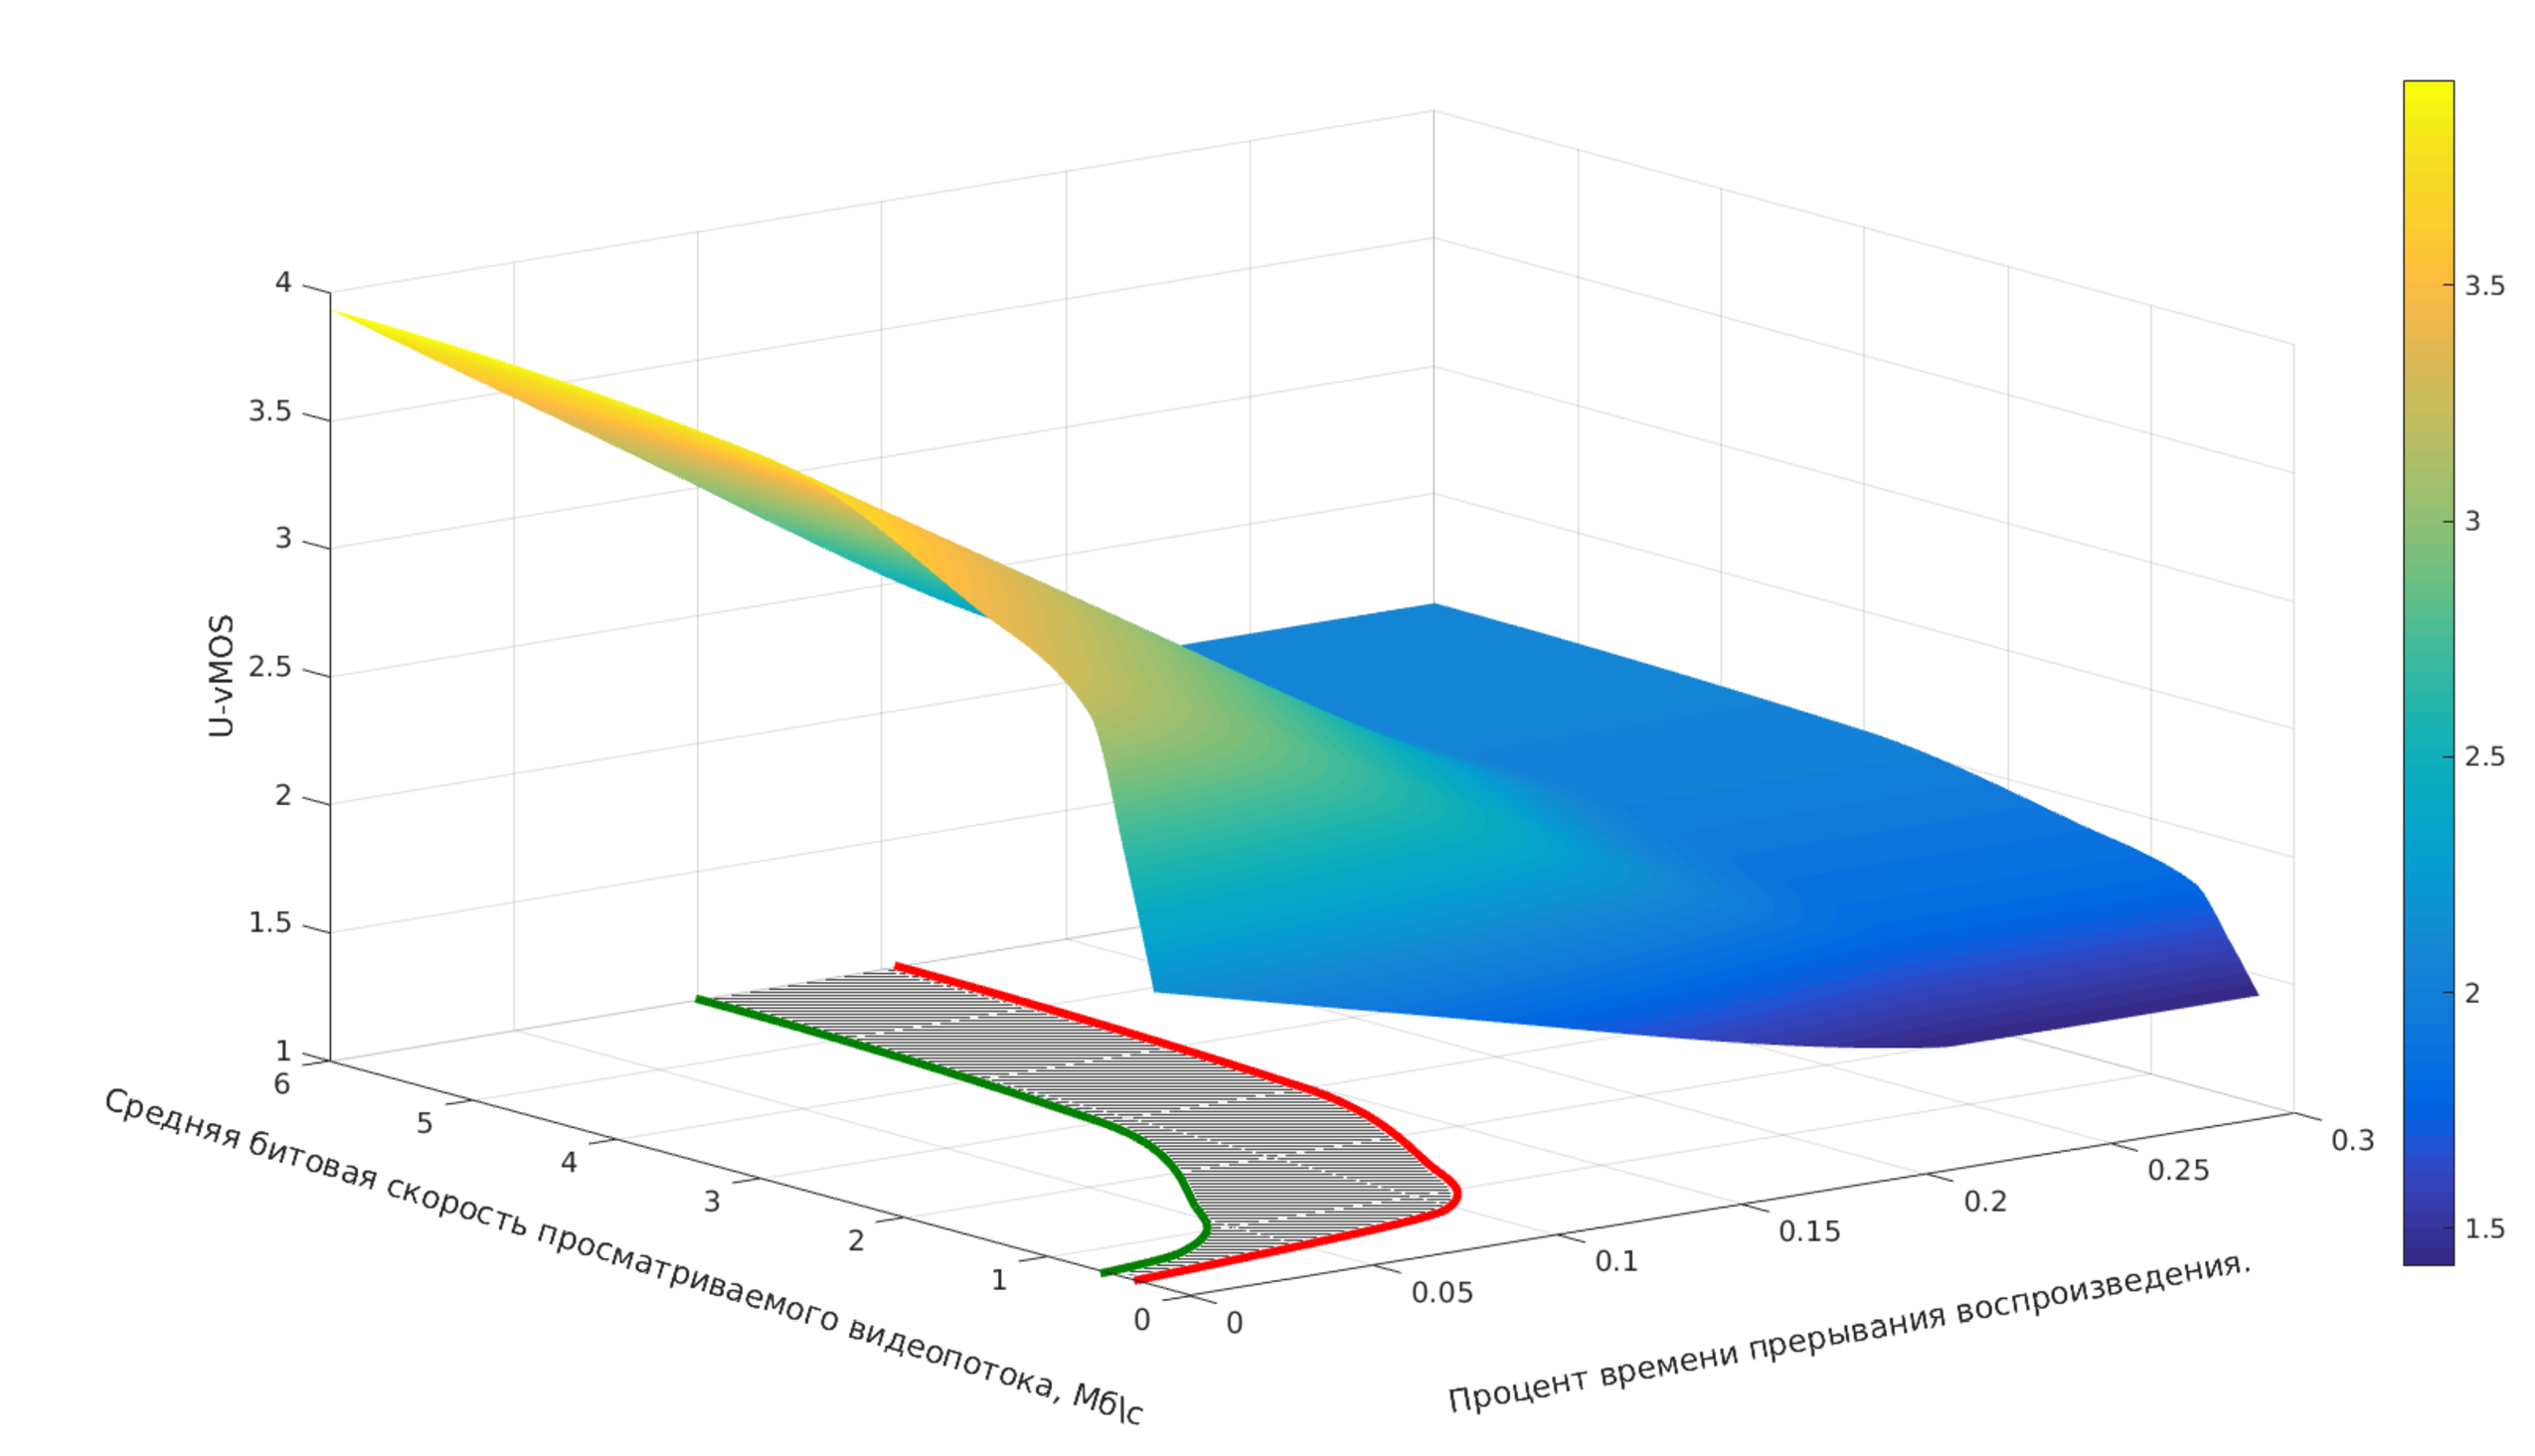
\includegraphics[width=\textwidth]{Chapter1/mos_figure.pdf}
\caption{Влияние объективных характеристик на критерий качества восприятия U-vMOS}
\label{fig:UvMOSDepending}
\end{center}
\end{figure}

По оси абсцисс отложена средняя битовая скорость просматриваемого видео, по оси ординат средний процент времени прерывания воспроизведения видео (повторные буферизации) и ось аппликат представляет результат вычисления критерия качества восприятия U-vMOS, при заданных параметрах. Процесс управлением полезной скорость передачи данных, во время просмотра видео, может привести в одну из возможных точек полученной плоскости. Значения по оси аппликат находятся в диапазоне от одного до четырех, разделим плоскость на три области:
\begin{itemize}
  \item Область высокого значения критерия восприятия (левее заштрихованной области) соответствует значениям в выше 3-х. Если пользователю была обеспечена полезная скорость для попадания в данную область, то он будет удовлетворен качеством обслуживания.
  \item Граничная область (заштрихованная область) соответствует значениям в отрезке от 2.5 до 3-х. Граничная область характеризует пограничное состояние удовлетворенности пользователя.
  \item Область низкого значения критерия восприятия (правее заштрихованной области) соответствует значениям в ниже 2.5. В данной области полезной скорости недостаточно для обеспечения достойного уровня обслуживания, таким образом пользователь считается неудовлетворенным.
\end{itemize}

Целью управления, увеличивающего производительность телекоммуникационной сети, является максимизация чила пользователей, находящихся в области высокого значения критерия восприятия. Это может быть достигнуто путем перераспределения ресурсов системы для пользователей в граничной области, за счет пользователей в области низкого значения критерия, так как перераспределение ресурсов для них не может привести к увеличению их удовлетворенности. Подобный анализ может быть проведен для любого критерия качества восприятия, представленего в подразделе~\ref{chap1:VideoMOS}.

\section{Выводы по разделу}

В качестве выводов по разделу можно отметить, что задача анализа и увеличения производительности телекоммуникационных сетей для передачи видеоданных является актуальной, ввиду бурного развития мобильных устройств. Основной целью увеличения производительности сетей является максимизация числа видеопользователей, одновременно активных в сети. Данная цель может быть достигнута путем введения управления полезной скоростью передачи данных, которое основывается на знании о формате представления видеоданных при передаче (подраздел~\ref{chap1:VideoFormat}), особенностей организации передачи видео и типах воспроизводящих устройств (подраздел~\ref{chap1:VideoPlayers}), объективных, субъективных показателей качества обслуживания и их взаимосвязи (подразделы~\ref{chap1:VideoMOS} и~\ref{chap1:InterrelationKPIandQoE} соотвественно).

Увеличение производительности телекоммуникационных систем для передачи видеоконтента является особенно актуальным для мобильных сетей связи, ввиду ограниченности ресурсов и динамичности состояния беспроводного канала.

В качестве основных результатов стоит отметить следующие:
\begin{itemize}
	\item В настоящее время существуют две технологии доставки видеоданных по протоколу HTTP: неадаптивная и адаптивная (подраздел \ref{chap1:VideoPlayers});
	\item Оценка качества восприятия видеоданных является сложной задачей ввиду субъективности пользователя, и более того зависит от технологии передачи видео (подраздел \ref{chap1:VideoMOS});
	\item Основные факторы, влияющие на качество восприятия видеопотока в зависимости от технологии передачи (подраздел \ref{chap1:InterrelationKPIandQoE}):
	\newline\textbf{Неадаптивная технология}~--~длительность буферизации в период просмотра видео;
	\newline\textbf{Адаптивная технология}~--~длительность буферизации и битовая скорость просматриваемого потока.
\end{itemize}

Информация, представленная в данном разделе, во многом носит обзорный характер, с использованием методов обратной разработки и анализа <<черного ящика>>. Представленное исследование демонстрирует основную проблематику передачи видео в телекоммуникационных системах и является основополагающим для последующих разделов работы.